\section{Synthesis and test on FPGA}
\label{sec:synthezisResults}
The results from synthesizing in Vivado can be seen in \cref{tab:cell_usage}, \cref{tab:resource_utilization} and \cref{fig:utilization}. The area requirement of less than 50 \% resource use is fulfilled in the Vivado synthesis, with a usage at around 22 - 24 \%. From \cref{tab:fpga_performance} one can see that the demands are met on the FPGA server as well. The number of logic cells used is less on the FPGA server. This might be because of different FPGA technologies or different optimizations during synthesis. The requirement to reach a target frequency of 50 Mhz is fulfilled with a max frequency of 56.95 Mhz on the FPGA server, see \cref{tab:fpga_performance}.

Due to some issues with setting up correct constraints in Vivado, the worst negative slack was reported to be inf. A clear sign that something in the constraints were wrong. Therefore the calculation to get max frequency after Vivado synthesis could not be executed.

The number of average clock cycles per block from the FPGA server (\cref{tab:fpga_performance}) is 42512. This number is less than the worst-case calculations in \cref{sec:estimatePerfArea} and close to the other calculations. The estimate of the area is a bit off, but only by a small amount. The estimate was around 2186 LUTs and the actual number differs between 2833 and 1662 LUTs.

As a proof that it is actually working, the output from the FPGA server can be found in \cref{app:fpga_output}, and the result after countless sleepless nights can be seen in \cref{fig:rocket}

%\todo[inline]{Get WNS from vivado using  constraints}
%\todo[inline]{litt tynt. Kunne vært mer tekst her!}
%\inputminted[linenos=0, firstline=82, lastline=102, frame=none]{text}{../RSA/synthesis_report.txt}
%\inputminted[linenos=0, firstline=309, lastline=318, frame=none]{text}{../RSA/synthesis_report.txt}
%
\begin{table}[htp]
    \begin{center}
        \begin{tabular}{l | r}
            Instance                     & Cells \\
            \hline
            Total RSA                    & 2833 \\
            \quad monpro                 & 1428 \\
            \qquad u\_monpro\_controller & 293  \\
            \qquad u\_monpro\_datapath   & 1135 \\
            \quad u\_rsa\_controller     & 74   \\
            \quad u\_rsa\_datapath       & 1261 \\
        \end{tabular}
        \caption{Cell usage divided by instances}
        \label{tab:cell_usage}
    \end{center}
\end{table}
%
\begin{table}[htp]
    \begin{center}  
        \begin{tabular}{ l | c | c | r}
             Resource & Utilization & Available & Utilization \%  \\
             \hline
             Slice LUTs & 1024 & 218600 & 0.47 \\
             Slice Registers & 1245 & 437200 & 0.28 \\
             IO & 69 & 362 & 19.06 \\
             Clocking & 1 & 32 & 3.12 \\
        \end{tabular}
        \caption{Summary of resource utilization }
        \label{tab:resource_utilization}
    \end{center}
\end{table}
%
\begin{figure}[htp]
    \centering
    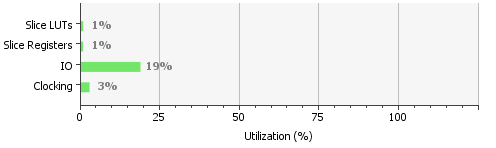
\includegraphics[width=0.6\textwidth]{images/utilization}
    \caption{A graph over the utilization of the various resources}
    \label{fig:utilization}
\end{figure}

\begin{figure}
    \centering
    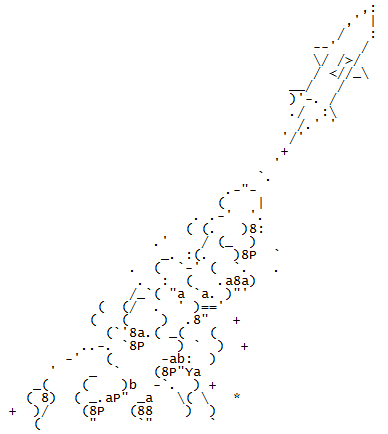
\includegraphics[width=0.3\textwidth]{images/rocket}
    \caption{Output from test on the FPGA}
    \label{fig:rocket}
\end{figure}
%
\begin{table}[htp]
    \begin{center}
        \begin{tabular}{l | r}
            Property              & Value              \\
            \hline
            Avg. cycles per block & 42512              \\
            Number of latches     & 0                  \\
            Logic cells used      & 1662               \\
            fmax                  & 56.95 MHz          \\
            Throughput            & 1340 blocks/second \\
        \end{tabular}
        \caption{Performance output from FPGA test}
        \label{tab:fpga_performance}
    \end{center}
\end{table}
